%保存为UTF-8编码格式
%用xelatex编译
 
\documentclass[UTF8,a4paper,12pt]{ctexart}
\usepackage[left=2.50cm, right=2.50cm, top=2.50cm, bottom=2.50cm]{geometry} %页边距
\CTEXsetup[format={\Large\bfseries}]{section} %设置章标题字号为Large,居左
%\CTEXsetup[number={\chinese{section}}]{section}
%\CTEXsetup[name={(,)}]{subsection}
%\CTEXsetup[number={\chinese{subsection}}]{subsection}
%\CTEXsetup[name={(,)}]{subsubsection}
%\CTEXsetup[number=\arabic{subsubsection}]{subsubsection}  %以上四行为各级标题样式设置,可根据需要做修改
 
%\linespread{1.5} %设置全文行间距
 
 
%\usepackage[english]{babel}
%\usepackage{float}     %放弃美学排版图表
\usepackage{fontspec}   %修改字体
\usepackage{amsmath, amsfonts, amssymb} % 数学公式相关宏包
\usepackage{color}      % color content
\usepackage{graphicx}   % 导入图片
\usepackage{subfigure}  % 并排子图
\usepackage{url}        % 超链接
\usepackage{bm}         % 加粗部分公式,比如\bm{aaa}aaa
\usepackage{multirow}
\usepackage{booktabs}
\usepackage{epstopdf}
\usepackage{epsfig}
\usepackage{longtable}  %长表格
\usepackage{supertabular}%跨页表格
\usepackage{algorithm}
\usepackage{algorithmic}
\usepackage{changepage}
\usepackage[colorlinks,linkcolor=blue]{hyperref}
\usepackage{graphicx}
\usepackage{subfigure}
\usepackage{float}
\usepackage{pdfpages}
 
 
 
%%%%%%%%%%%%%%%%%%%%%%%
% -- text font --
% compile using Xelatex
%%%%%%%%%%%%%%%%%%%%%%%
% -- 中文字体 --
%\setCJKmainfont{Microsoft YaHei}  % 微软雅黑
%\setCJKmainfont{YouYuan}  % 幼圆
%\setCJKmainfont{NSimSun}  % 新宋体
%\setCJKmainfont{KaiTi}    % 楷体
\setCJKmainfont{SimSun}   % 宋体
%\setCJKmainfont{SimHei}   % 黑体
 
% -- 英文字体 --
\setmainfont{Times New Roman}
%\setmainfont{DejaVu Sans}
%\setmainfont{Latin Modern Mono}
%\setmainfont{Consolas}
%
%
\renewcommand{\algorithmicrequire}{ \textbf{Input:}}     % use Input in the format of Algorithm
\renewcommand{\algorithmicensure}{ \textbf{Initialize:}} % use Initialize in the format of Algorithm
\renewcommand{\algorithmicreturn}{ \textbf{Output:}}     % use Output in the format of Algorithm
\renewcommand{\abstractname}{\textbf{\large {摘\quad 要}}} %更改摘要二字的样式
\newcommand{\xiaosi}{\fontsize{12pt}{\baselineskip}}     %\xiaosi代替设置12pt字号命令,不加\selectfont,行间距设置无效
\newcommand{\wuhao}{\fontsize{10.5pt}{10.5pt}\selectfont}
 
\usepackage{fancyhdr} %设置全文页眉、页脚的格式
\pagestyle{fancy}
\lhead{}           %页眉左边设为空
\chead{}           %页眉中间
\rhead{}           %页眉右边
%\rhead{\includegraphics[width=1.2cm]{1.eps}}  %页眉右侧放置logo
\lfoot{}          %页脚左边
\cfoot{\thepage}  %页脚中间
\rfoot{}          %页脚右边
 
 
%%%%%%%%%%%%%%%%%%%%%%%
%  设置水印
%%%%%%%%%%%%%%%%%%%%%%%
%\usepackage{draftwatermark}         % 所有页加水印
%\usepackage[firstpage]{draftwatermark} % 只有第一页加水印
% \SetWatermarkText{Water-Mark}           % 设置水印内容
% \SetWatermarkText{\includegraphics{fig/ZJDX-WaterMark.eps}}         % 设置水印logo
% \SetWatermarkLightness{0.9}             % 设置水印透明度 0-1
% \SetWatermarkScale{1}                   % 设置水印大小 0-1
 
\usepackage{hyperref} %bookmarks
\hypersetup{colorlinks, bookmarks, unicode} %unicode
 
 
 
\title{\textbf{\Large{PMT测量方案}}}
\author{ 徐彤\quad 陈晖有\quad 赵林 }
\date{\today}
 
 
 
\begin{document}
 
\maketitle
%\tableofcontents
 
\begin{abstract}
PMT是高能物理实验中的一种重要仪器设备,世界上许多先进的粒子物理实验,比如中国的大亚湾,江门,锦屏中微子实验及日本的SuperK,韩国的RENO实验等等均需要应用到PMT进行数据测量。并且根据实验设计,对PMT的性能有一定的要求。这里介绍了测量PMT的峰谷比(P/V值),增益,渡越时间及离散程度(TTS),量子效率(QE),暗噪声率(Darknoise rate)等重要特性的测量方案及结果,以供参考。
\end{abstract}
 
\section{\textbf{实验设备}}
\subsection{光电倍增管(PMT)}
待测量设备为北方夜视生产的8英寸微通道板型PMT。8英寸的PMT为新产品,北方夜视官方仅提供了20英寸PMT的测量结果,具体参数可参见\href{http://ysgf.norincogroup.com.cn/art/2020/3/23/art_1235_25349.html}{北方夜视官网}。
\begin{figure}[H]
	\centering
	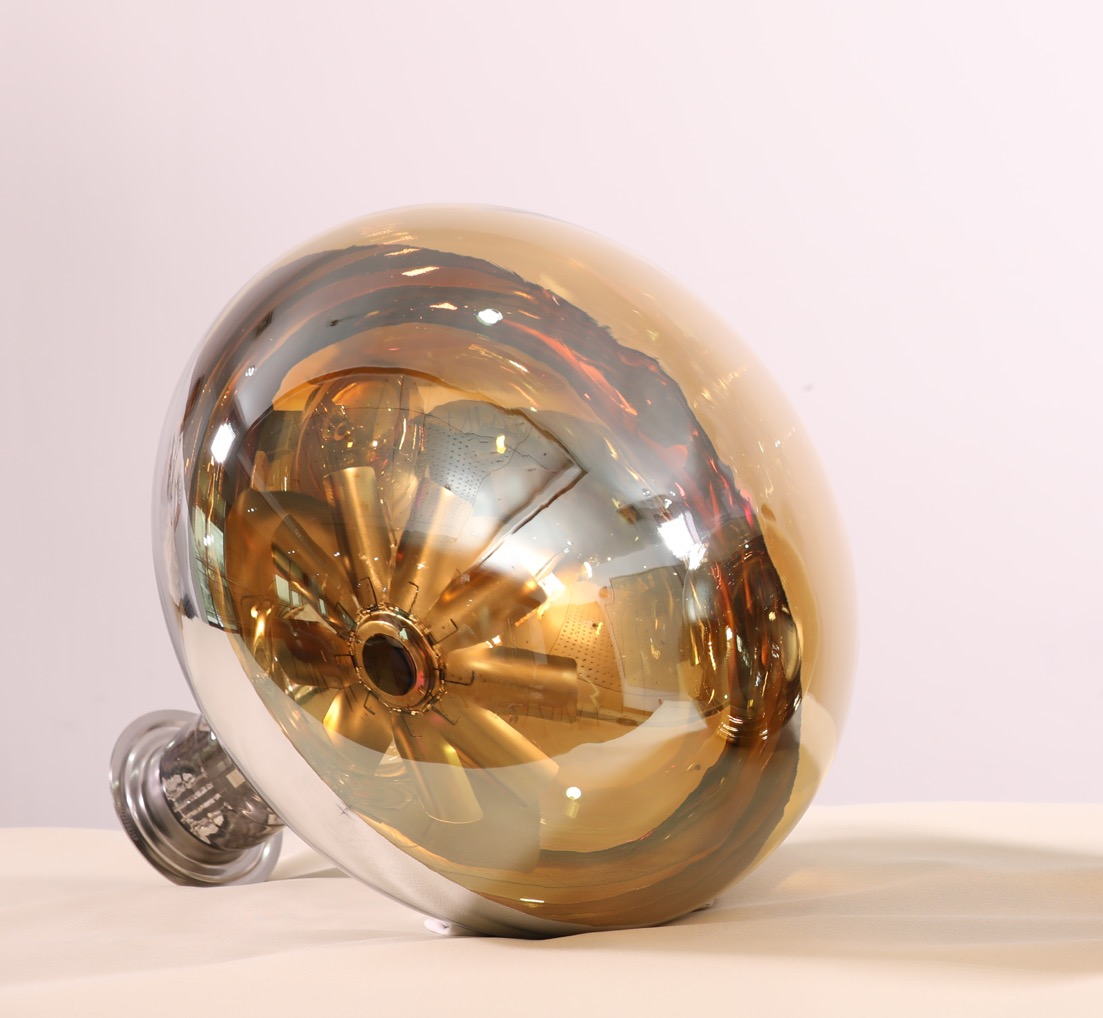
\includegraphics[width=0.5\linewidth]{20inch_PMT}
	\caption[图1]{20英寸PMT}
\end{figure}
\begin{figure}[H]
	\centering
	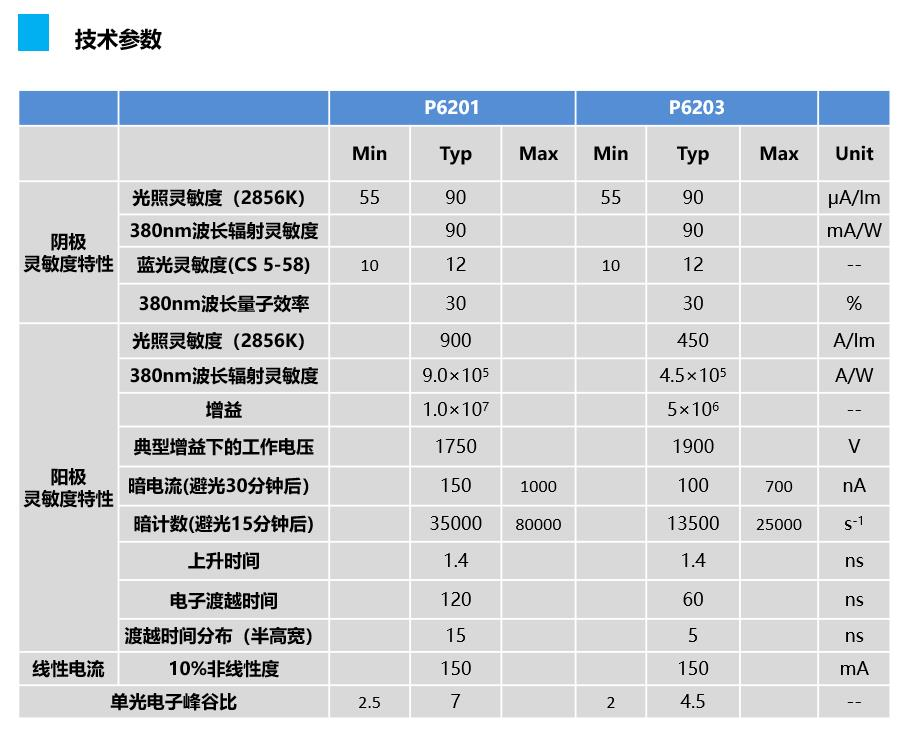
\includegraphics[width=0.8\linewidth]{技术参数}
	\caption[图2]{20 inch PMT技术参数表}
\end{figure}

\subsection{高压电源} 
高压电源主要给PMT管供电。要求电压源稳定供电电压范围在1700 V-2000 V,涵盖PMT的典型工作电压。需要考虑PMT供电电压的正负性,这里供电电压为正。
\begin{figure}[H]
	\centering
	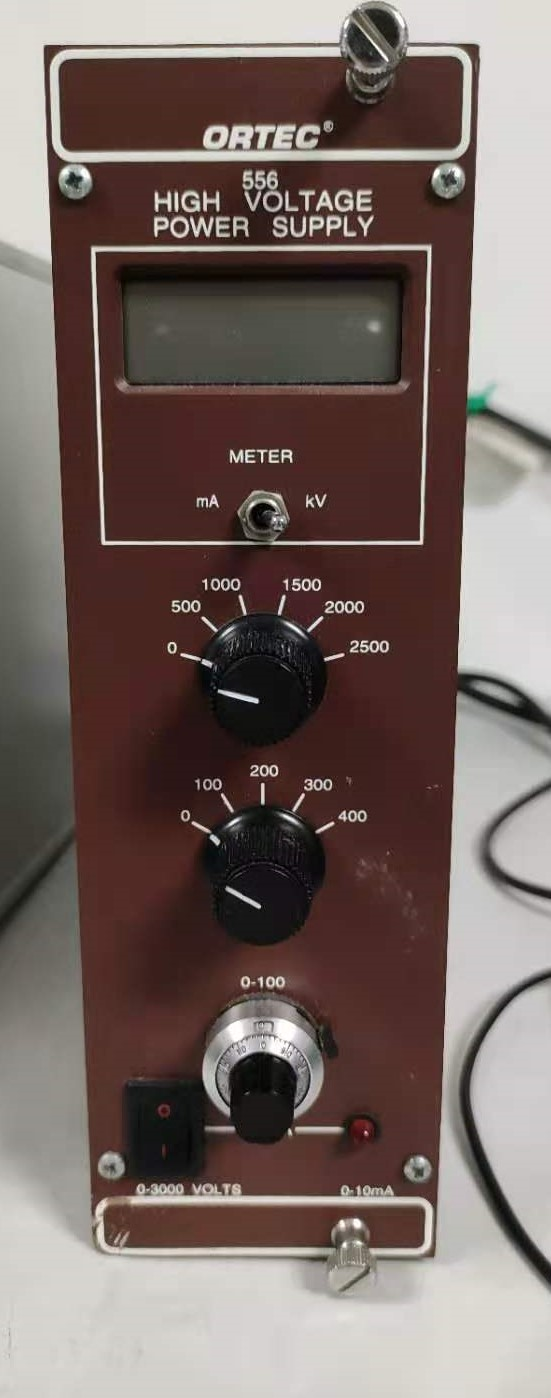
\includegraphics[width=3cm,height=7cm]{高压电源}
	\caption[图3]{高压电源}
\end{figure}

\subsection{采数设备}
采数设备主要用于PMT输出信号的读出。需要的设备有同轴信号线,快速模数转换插件(FADC),VME机柜,与电脑一台。\par
这里使用的VME机柜与FADC均为CAEN公司产品,其中VME机柜主要与FADC配套使用的具体参数可以参考\href{https://www.caen.it/search/VME}{CAEN VME}。FADC采用V1751,具体参数和使用说明可参考\href{https://www.caen.it/products/v1751/}{CAEN V1751}。

\subsection{其他实验设备}
PMT特性测量还用到一些其他的设备。\par
1. 暗室一个:主要是屏蔽光,为了测量PMT的暗特性,比如暗噪声率等等。箱体内部有信号线接口,信号的输入输出均经过信号接口,提高遮光效果。\par
2. 激光器:作为光源,可以产生不同波长的光线,并且有单光子模式,即光子可以单个发出。方便测量PMT的光学特性比如量子效率等等\par
3. 光纤:与激光器配套使用,注意光纤的变化,比如弯折或者位移等都可能导致输出光强度的变化。\par
4. 光罩:特殊设计的光罩,与光子发生器配套使用,使得PMT的特定位置接受到光子,方便测量空间特性。\par

\begin{figure}[H]
	\centering
	\subfigure[暗室]{
		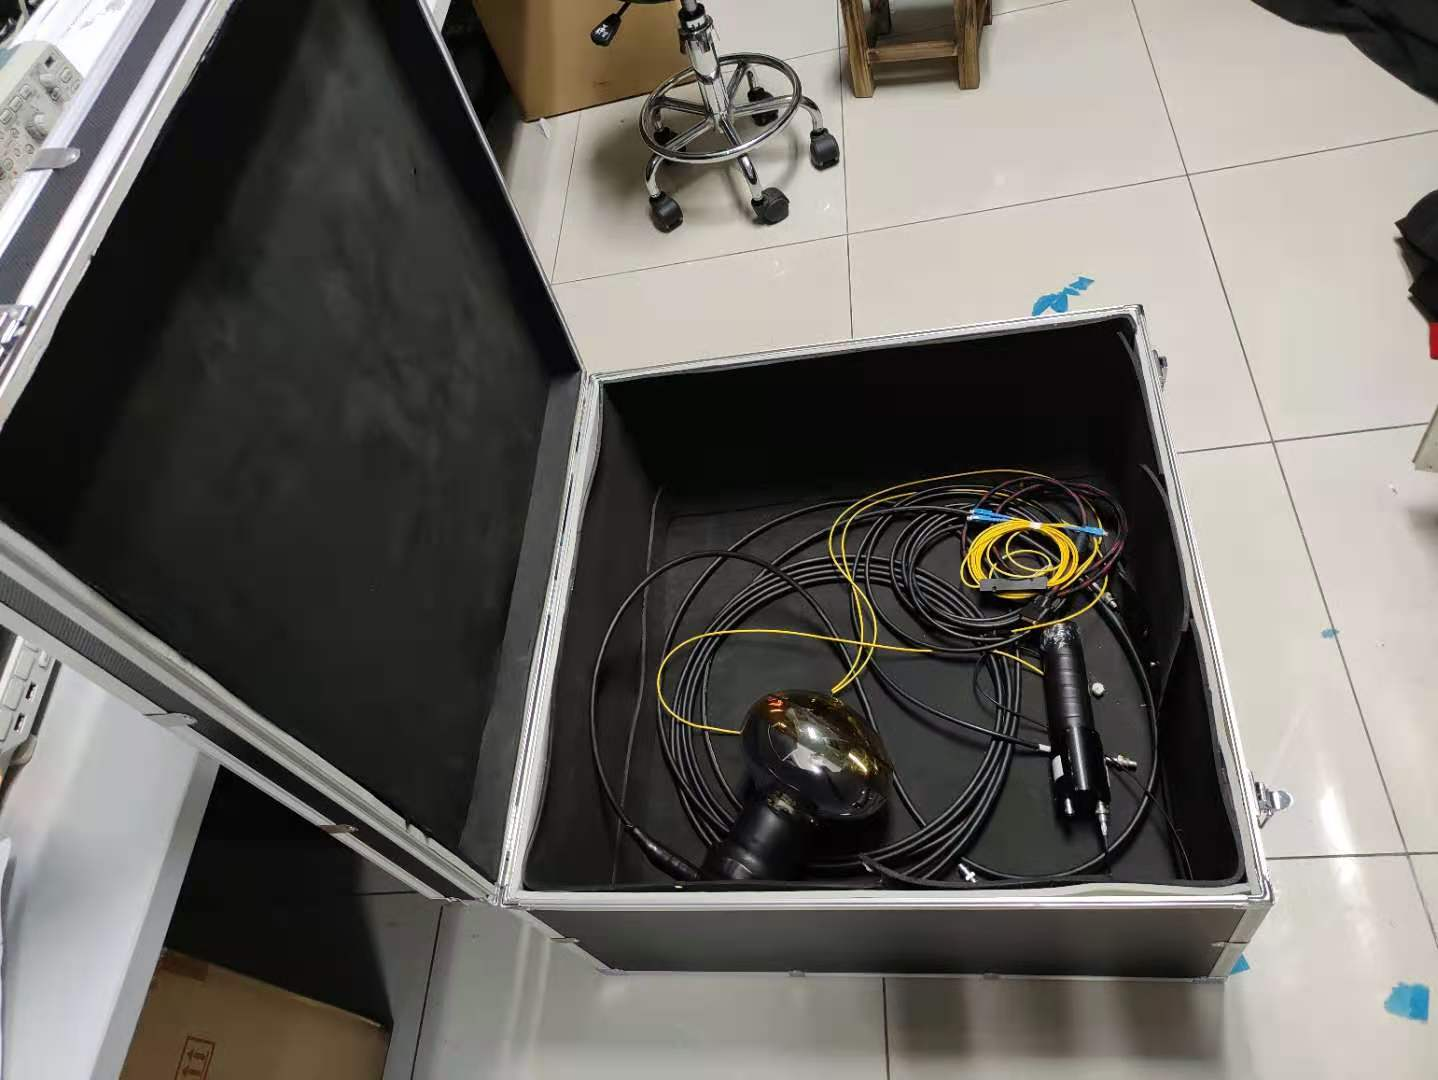
\includegraphics[width=0.4\linewidth,height=4.5cm]{暗室} \label{1}
	}
	\quad
	\subfigure[激光器]{
		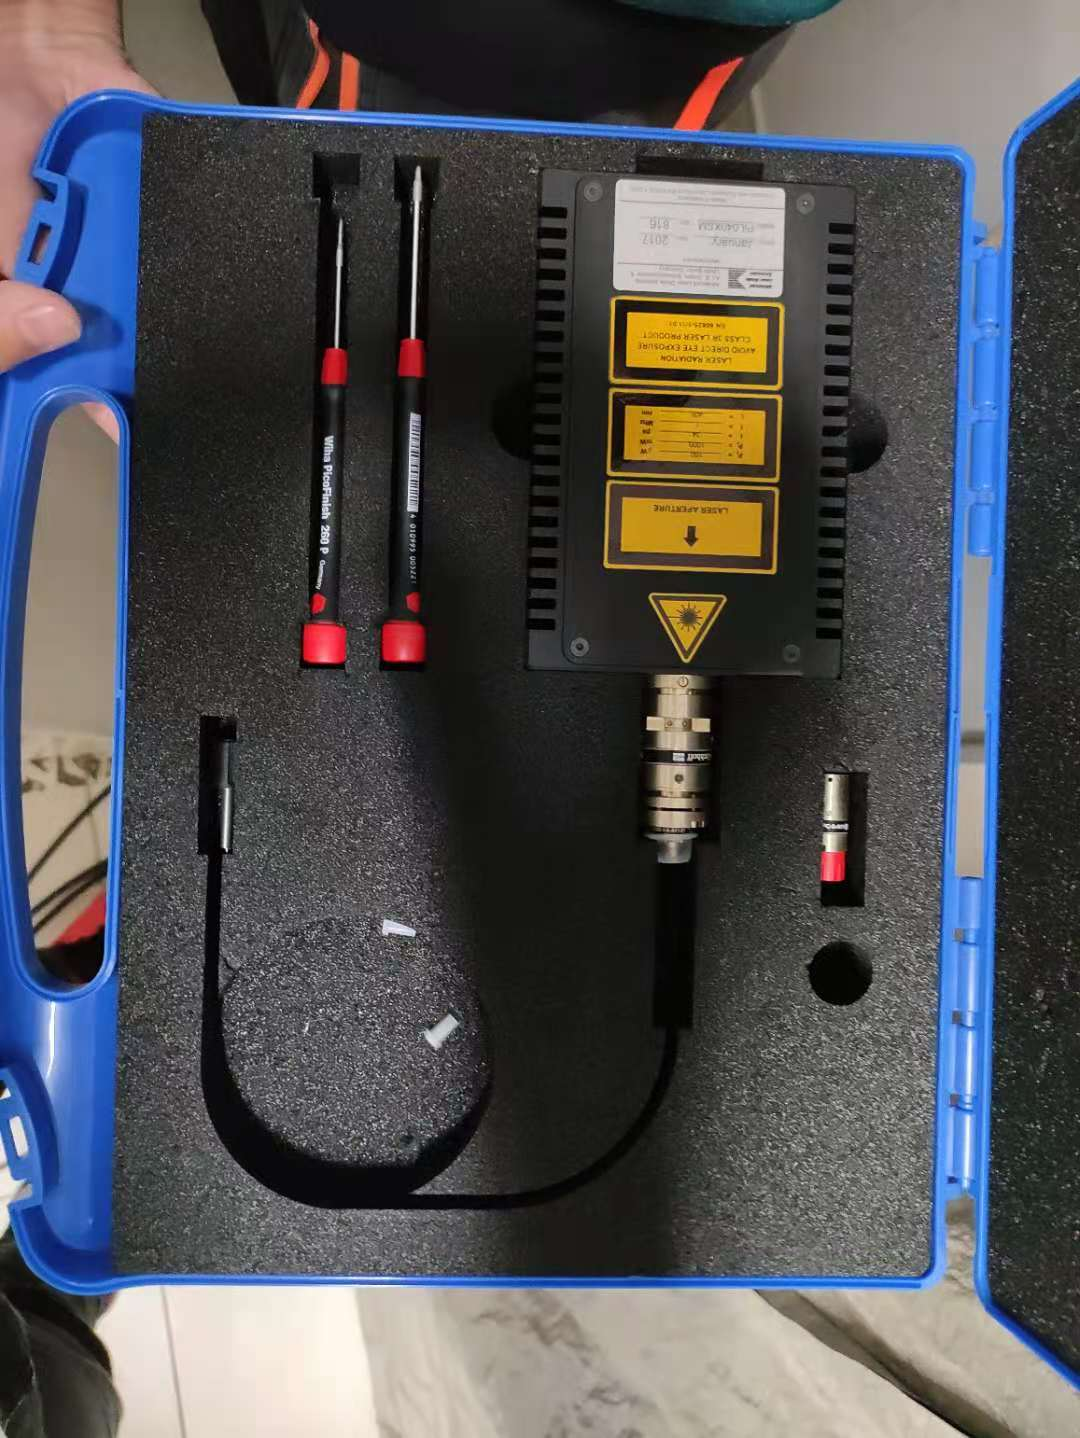
\includegraphics[width=0.4\linewidth,height=4.5cm]{激光器} \label{2} 
	}
	\quad
	\subfigure[光线]{
		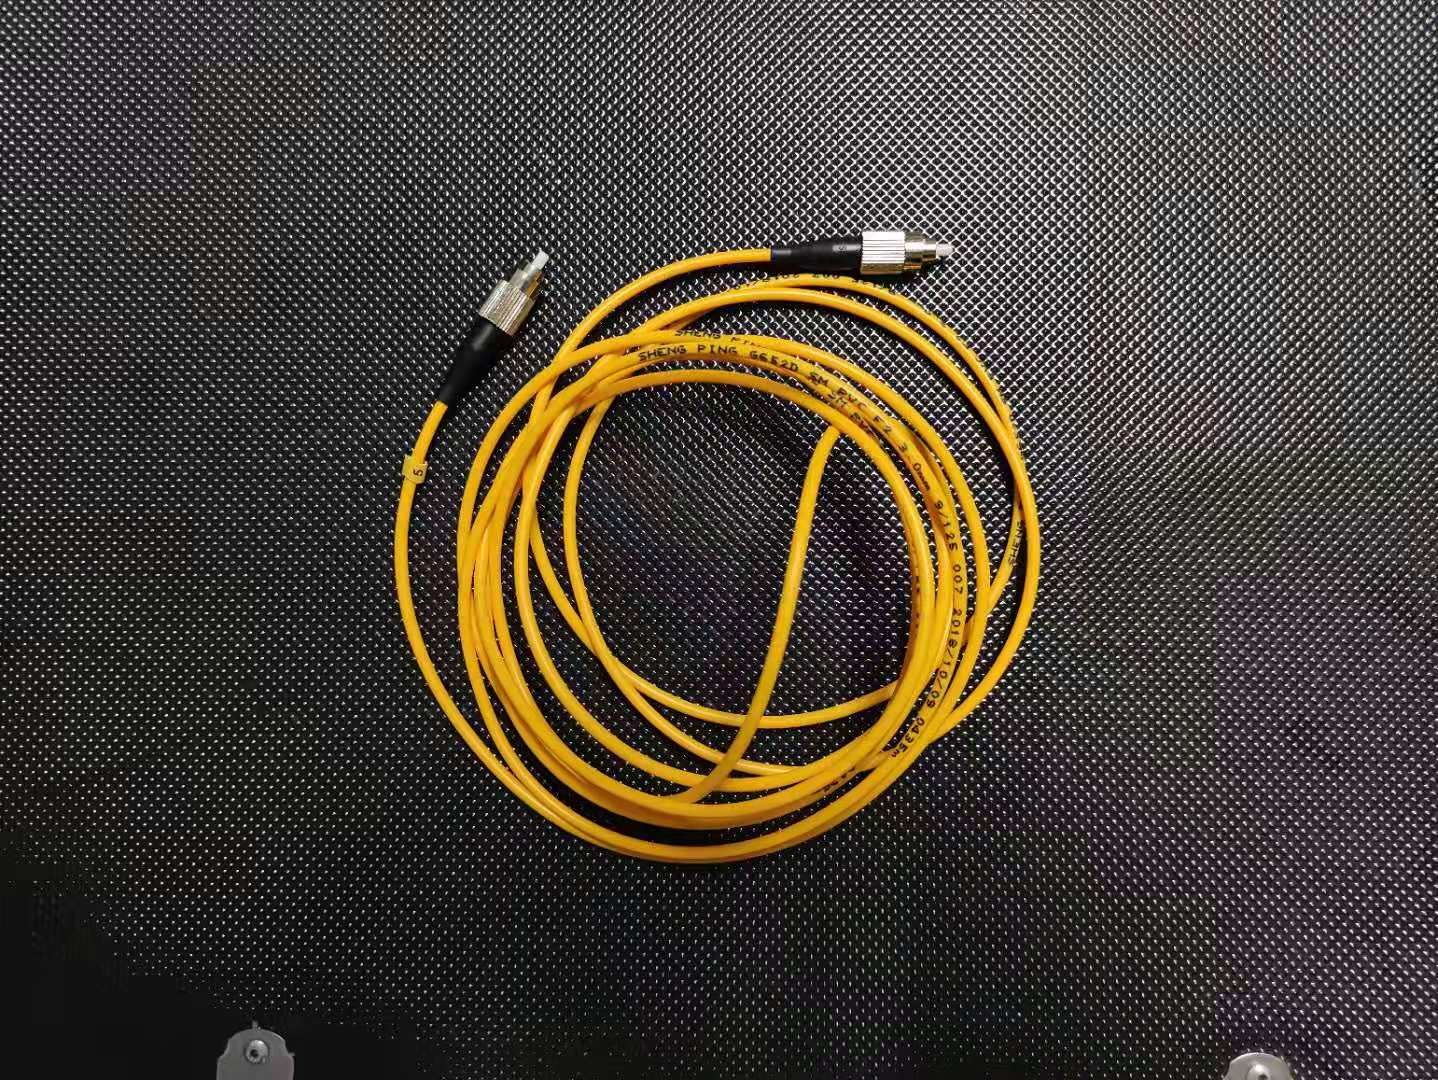
\includegraphics[width=0.4\linewidth,height=4.5cm]{光纤}\label{3}
	}
	\quad
	\subfigure[光罩]{
		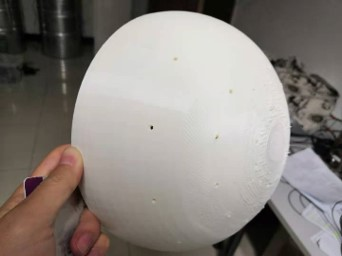
\includegraphics[width=0.4\linewidth,height=4.5cm]{光罩}\label{4}
	}
	\caption[图4]{其他实验设备}
\end{figure}


\section{增益、峰谷比、暗噪声率测量}
将PMT在黑箱中静置半小时以上,暗噪声速率逐渐下降区域稳定值[PMT光阴极在光照下会活化,暗噪声率提高]。注意用黑布遮住黑箱,防止外部光子进入。\par
利用FADC V1751,将PMT输出信号直接接入通道[如CH1],采用外部随机触发,运行采数程序开始采数。\par
考虑到官方给出的暗噪声的频率约为10k量级,即0.1ms量级。这对采样的频率以及时间窗口的长度有要求:\par
1.	时间窗口取1000ns,保证在一个窗口出现两个事例的概率几乎为0.\par
2.	采样频率取10Hz。\par
对采集的数据进行分析,得到其中暗噪声的计数,及其峰值和累积电荷的分布情况,得到PMT的增益、P/V值和Dark noise rate等特征值。\par
对信号电荷进行积分的两种方法:\par
1.  直接对全部信号进行积分,log scale可以看到单光电子的峰;\par
2.  先进行寻峰,然后再积分峰位附近电荷。\par
暗噪声计算方法有两种:\par
1.  寻峰方法,直接计数。\par
2.  对电荷积分结果进行拟合后,对1PE的信号积分求个数。\par

\section{QE和QE vs Position测量}
实验主要需要测量PMT对应于不同波长光下的量子效率(QE),以及典型波长下PMT光阴极不同位置的量子效率。\par
注意这里测量的量子效率为相对量子效率,需要加入参考PMT管。\par
注意光纤的变化,比如弯折或者位移等都可能导致输出光强度的变化。所以在测量过程中要尽量保证光输出的稳定性,并且进行检验校准。\par
测试电路的逻辑图和简单测量步骤如下:\par
\begin{figure}[H]
	\centering
	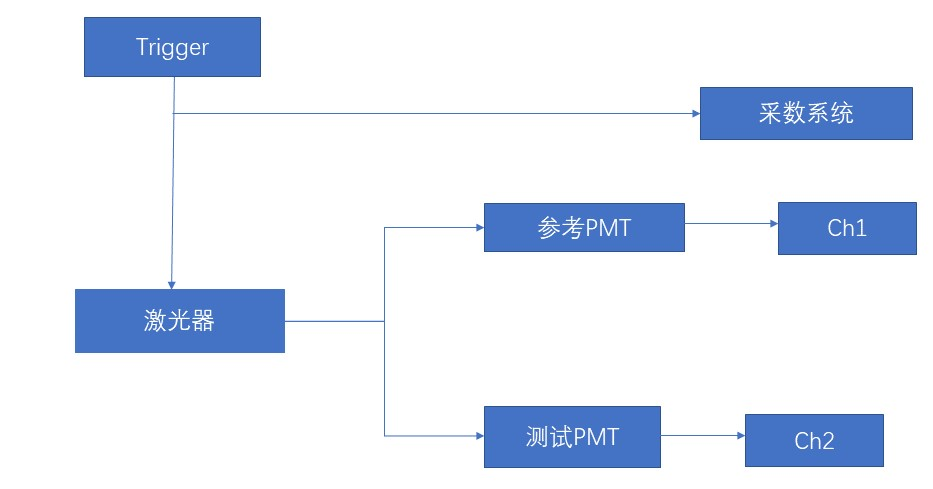
\includegraphics[width=0.8\linewidth,height=5.5cm]{QE测量逻辑.jpg}
	\caption[图5]{QE测试电路逻辑}
\end{figure}
测试步骤:\par
1. 激光器通过分光光纤分成两束;\par
2. 每一束通过同一PMT测试,校准两路光强$I_1/I_2$, 光强校准后保证光纤位置不动,否则会影响光强;\par
3. 测试两路信号,对测试结果的电荷进行积分;\par
4. 根据$QE_2=\frac{I_1nPE_2}{I_2nPE_1}\times QE_1$,得到测试PMT的相对量子效率。
\section{TTS和TTS vs Position测量}
实验主要需要测量PMT的渡越时间(TT),以及其离散程度(TTS)。\par
注意这里的激光器需要调整到单光子模式。\par
注意光纤的变化,比如弯折或者位移等都可能导致输出光强度的变化。所以在测量过程中要尽量保证光输出的稳定性,并且进行检验校准。\par
测量逻辑图如下:\par
\begin{figure}[H]
	\centering
	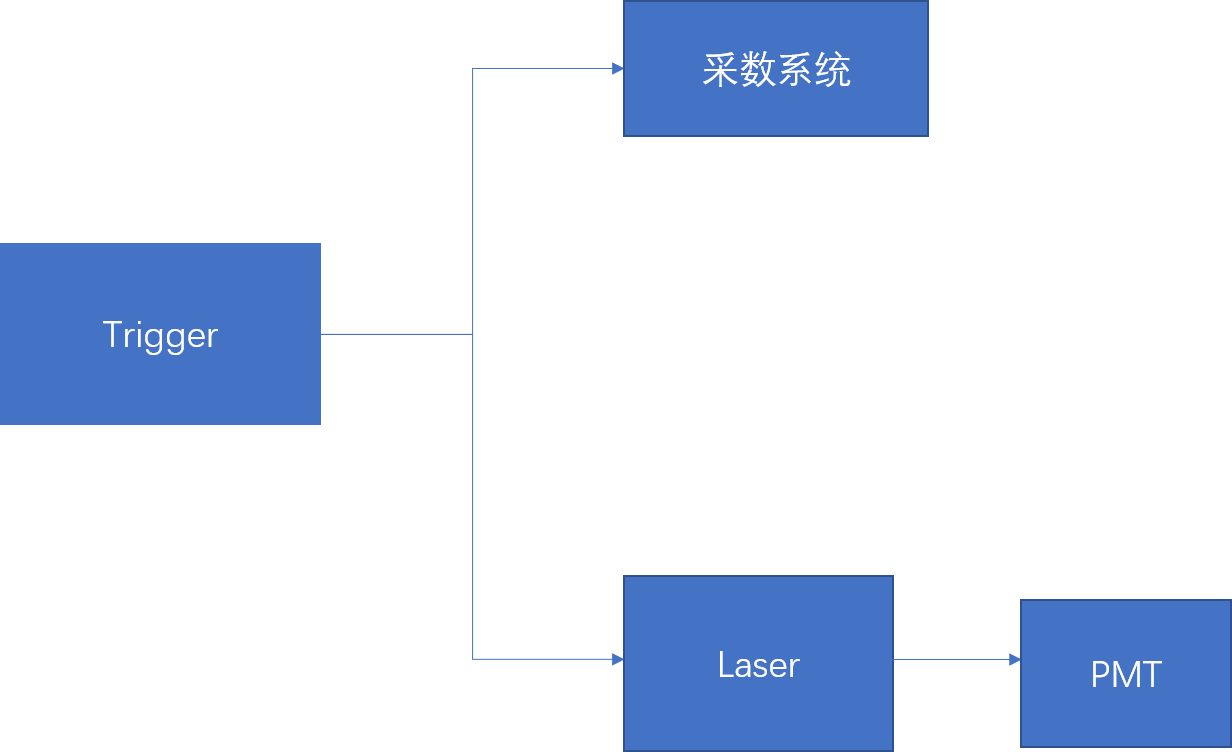
\includegraphics[width=0.8\linewidth]{TTS测量逻辑}
	\caption[图6]{TTS测试电路逻辑}
\end{figure}
图中Trigger可以为信号发生器产生,也可以为激光器产生。测试步骤如下:\par
1. 调整激光器光强,使其降低到单光子模式;\par
2. 采数为外部触发逻辑;\par
3. 两路同时记录触发时间和PMT信号;\par
4. 分析得到触发时间和PMT信号之间的时间差,该时间差为激光器光发射时间+光纤中传播时间+PMT渡越时间,忽略前两项展宽,该时间差的展宽可以近似为PMT的TTS。\par
注意激光器调整方式:\par
1. 该激光器无法直接调整到单光子模式;\par
2. 通过调整光纤接口和激光器出光口的夹角,使少量光可以进入光纤传播,以达到单光子效果。\par

\section{总体注意事项}
1. 注意实验室基本安全,严格按照操作规范进行操作;\par
2. 实验中一定要佩戴橡胶手套(不要污染PMT)、护目镜(防止PMT爆炸伤到眼睛);\par
3. PMT轻拿轻放,必须双手拿PMT。\par
4. 注意线缆、光纤的整齐,以及不可压到线缆。连接暗室通过暗室的接口进出线缆。\par

 
\end{document}